\documentclass[journal]{IEEEtran}
\usepackage{amsmath,amssymb}
\usepackage{booktabs}
\usepackage{graphicx}
\usepackage{hyperref}
\usepackage{multirow}

% ---- Anonymization toggle (paper-1 convention) ----
\newif\ifanonymous
\anonymoustrue

\ifanonymous
\newcommand{\repourl}{\url{https://anonymous.4open.science/status/moba-draft-policies}}
\newcommand{\deployurl}{\url{https://draft-assistant-review.vercel.app}}
\else
\newcommand{\repourl}{\url{https://github.com/maxsegan/moba-draft-policies}}
\newcommand{\deployurl}{\url{https://www.hotsfever.com}}
\fi
% ---- Pre-registration (OSF 3cxvd, registered 2026-09-27, embargoed to 2027) ----
\newcommand{\preregdate}{September 27, 2026}
\ifanonymous
\newcommand{\prereglink}{\url{https://osf.io/3cxvd/overview?view_only=dbe817f56afe4507865e44bf24510748}}
\else
\newcommand{\prereglink}{\url{https://osf.io/3cxvd}}
\fi
% ---------------------------------------------------

% ==== Arm names as macros: "frozen" is never written bare. ====
\newcommand{\maintained}{\textsc{maintained}}          % cumulative-refresh agent
\newcommand{\maintainedpred}{\textsc{maintained-d90}}  % decayed-aggregate stats
\newcommand{\mcut}{\textsc{maintained-at-cutoff}}      % maintained VF, cutoff stats
\newcommand{\stalefour}{\textsc{unmaintained}}          % leak-free, cutoff-frozen
\newcommand{\leakyunm}{\textsc{unmaintained-leaky}}     % first version, self-inclusive stats
\newcommand{\staleone}{\textsc{stale-1yr}}
\newcommand{\staletwo}{\textsc{stale-2yr}}
\newcommand{\leakyfrozen}{\textsc{leaky-frozen}}
\newcommand{\capqm}{0.515 to 0.537}
\newcommand{\analysisdate}{to be stated here and on OSF at submission}
% ==============================================================

\begin{document}

\title{Maintaining Draft Policies Under Meta Drift:\\ What Retraining and Refresh Are Worth}
\ifanonymous
\author{Anonymous Authors}
\else
\author{Max~Segan and Hod~Lipson}
\fi
\maketitle

\begin{abstract}
Learned draft assistants deploy into games whose balance keeps changing.
Using 1.95 million ranked Heroes of the Storm drafts spanning 45 game
builds over 4.5 years, we measure what that drift costs a deployed draft
policy and what each kind of maintenance buys back. In a replayed
2.8-year deployment, a model that is never maintained loses 1.06
percentage points of accuracy against one retrained after every build.
Retraining every three builds recovers 1.01 of those points; recomputing
the model's aggregate statistics at every build, with the weights fixed,
recovers 0.33. Once retraining is on a schedule, refreshing statistics
between retrains adds only 0.02 to 0.04 points. Accuracy understates
policy differences: two training regimes within 0.03 points of each
other draft structurally broken teams at 17\% and 32\%. Head-to-head,
scored on 298{,}000 games from five later builds that no agent's
statistics include, a maintained agent's picks average 0.34 percentage
points more realized future-meta hero win rate than those of an agent
trained at the same cutoff ($p = 0.07$ with value-function seed variance
charged). The same-cutoff gap is consistent with how the value model
was trained; three months of refreshed statistics add nothing
measurable at the agent level. With opponent models matched by era, an
agent trained at the 2026 cutoff leads agents trained one and two years
earlier by 0.97 and 0.64 points. An outcome-shift
detector fires on 16 of 21 build boundaries with documented changes and
on 1 of 6 without (Fisher $p = 0.015$), yet as a refresh trigger it does
no better than a calendar. Learned judges drift too: every judge trained
before 2023 reverses the verdict of a 2026 contest.\footnote{\repourl}
\end{abstract}

\begin{IEEEkeywords}
Concept drift, dataset shift, MOBA drafting, model maintenance,
non-stationarity.
\end{IEEEkeywords}

\section{Introduction}

In prior work we built a draft assistant for Heroes of the Storm and
deployed it in a browser where anyone can draft against
it~\cite{paper1}. That paper froze the world on purpose: every
experiment ran on a snapshot of 1.95 million ranked drafts, pinned in
May 2026, so that results would be reproducible. The game did not hold
still. Across the window our corpus covers, the developer shipped 45
game builds, and the balance changes among them moved the meta under
every model we trained.

This paper restores the time axis and asks what a deployed draft policy
loses when nobody maintains it, and what each maintenance action buys
back. The two actions we price are retraining the model and refreshing
the aggregate statistics its features are computed from (hero, pair,
map, and composition win rates), with the weights left alone. Refresh is
nearly free; retraining costs a training run. Practitioners would like
to know whether the cheap action is enough.

We answer in four parts. First, a replayed 2.8-year deployment prices
both actions at the accuracy level. Never maintaining costs 1.06
percentage points (pp) of accuracy relative to retraining after every
build. Retraining every three builds recovers 1.01pp of that, and
refreshing statistics without retraining recovers 0.33pp. With retraining
on a schedule, refresh between retrains adds 0.02 to 0.04pp, and every
cadence from one to six builds lands within 0.11pp of retraining
constantly. Second, accuracy understates what drift does to policies.
Among eight training regimes, the patch-embedding regime comes within
0.03pp of our maintained model's future accuracy, yet drafting greedily
it assembles structurally broken teams twice as often (32\% against
17\%). Third, maintained and unmaintained MCTS agents draft against each
other and are scored against realized outcomes of games that no
agent's statistics include. Against an agent trained at the same cutoff, the maintained
agent's picks average +0.34pp of realized future-meta hero win rate
($p = 0.07$; +0.43pp, $p = 0.008$, with a single value function and more
agent seeds). That gap is consistent with training the value model on
statistics aligned with each game's era, and three months of refreshed
statistics add nothing measurable. Agents built with the same
value-function recipe one and two years earlier, each with an opponent
model of its own era, trail an agent trained at the 2026 cutoff by 0.97
and 0.64pp when that agent's opponent model is also of its era. Fourth, the machinery a maintainer needs around these
decisions: a detector of balance changes from outcomes alone, measured
against the developer's patch notes, and the observation that learned
judges age like the models they judge.

Scoping notes. Each learned judge we tried scores this contest by
its own era (Section~\ref{sec:vintage}), so the head-to-head results are
scored on realized future outcomes. And the
retrospective design can be tuned to the future it holds out, so we
registered forward tests on OSF before submission
(Section~\ref{sec:prospective}). Throughout, statistics used as training
features are computed causally or out of fold, because statistics that
include a row's own outcome leak its label into its features
(Section~\ref{sec:setting}).

\section{Setting, Corpus, and Names}
\label{sec:setting}

We use the pinned corpus of our earlier work: 1{,}943{,}338 ranked
Heroes of the Storm drafts on major patch 2.55, December 2021 through May
2026, a window over which the hero pool is fixed at 90. What is new is
the time structure. The corpus spans \textbf{45 game builds}, of which 28
have at least 20{,}000 games (``sizable''). The balance unit is the
build: hero tuning ships per build, and one marketing-level patch can
span many builds. Build counts recur in this paper, nested as follows. Of the 45
builds, 28 are sizable. Forty builds map to scripted patch notes, and
five have no published notes and are treated as no-change builds
(Section~\ref{sec:detect}). Consecutive sizable builds define 27
boundaries that are detectable in principle; the notes for 21 of them
mention at least one hero and the notes for 6 mention none. Skill is
bucketed into three tiers: low (Bronze and Silver), mid (Gold and
Platinum), and high (Diamond and Master); the 5{,}749 games without a
league tier are excluded. Replacing the tier one-hot with continuous average match
rating changes future accuracy by $-$0.017pp, and appending it changes
it by +0.007pp, both inside seed noise.

All value functions share the architecture of our earlier work: a
283-input MLP over hero identities, map, tier, and aggregate-statistic
features. The aggregate statistics come from our own corpus, per build
and cumulatively to each build. The temporal split is a hard cutoff at
build 2.55.14.95918 (February 2026). Training uses builds up to the
cutoff; the \emph{future window} is the seven strictly later builds,
about 144{,}000 games. Where statistics come from matters in this paper,
so we state it per arm. The \maintained{} recipe gives every row
statistics cumulative through the build before its own, which is causal
by construction. The cutoff-frozen recipes give deployment rows the
cumulative statistics at the cutoff, and their training rows the same
statistics computed out of fold, as described next. Accuracies are
labeled either
\emph{future-window} (the seven builds) or \emph{deployment-weighted} (a
2.8-year replay, Section~\ref{sec:replay}); the two windows give
different numbers for the same policy.

\textbf{Out-of-fold statistics.} Giving every training row the
statistics frozen at the cutoff leaks labels: a December 2021 game's
hero, pair, map, and composition win rates would then be computed from
every game through February 2026, including that game, a known hazard
with target statistics~\cite{kaufman2012leakage,prokhorenkova2018catboost}.
Each replay therefore receives one of five hash folds, and a training
row gets the cutoff statistics with its own fold's games removed;
deployment rows keep the unmodified cutoff statistics, which contain no
deployment game. Built from the full counts, the same code reproduces
the stored cutoff statistics to the last digit. The first version of
this study used the leaky construction for every cutoff-frozen arm, and
the correction changed results. For all-history training, in-period
validation accuracy falls from 59.04\% to 57.31\%, the calibration slope
on the future window (the slope of a logistic recalibration of the
model's predictions; 1 is calibrated) rises from 0.70 to 0.96
(\maintained{}: 0.92), and the rate of structurally broken teams
under greedy drafting falls from 43.5\% to 25.8\%. In-period validation
cannot reveal the leak, because validation rows carry it too; the leaky
models look calibrated there (slope 1.0). Because training rows see
statistics from four fifths of the games and deployment rows from all of
them, cells near the count thresholds could go missing more often in
training; on a 60{,}000-game sample the lookup rates differ by at most
0.007 percentage points. We report the leaky versions only as labeled
controls, next to the leak-free results they replace.

The agent under maintenance has three learned parts. A win-probability
model (the MLP above) scores completed drafts. An opponent model,
trained by behavioral cloning on human next-picks, supplies realistic
adversaries. A policy network, trained by AlphaZero-style Monte Carlo
tree search (MCTS) self-play against the opponent model with the
win-probability model at the leaves, proposes picks and bans; the search
kernel computes the win-probability features from a table of aggregate
statistics. Evaluation uses two instruments. Head-to-head drafting: two
agents alternate through the real 16-step ban-pick protocol, each acting
greedily from its policy head, and the terminal drafts are scored against
statistics of games actually played later (Section~\ref{sec:neglect}).
Structural metrics: the degenerate-composition rate counts teams missing
a role that role-level statistics show is required (a healer or a
frontline), and synergy and counter scores measure pairwise interactions
beyond hero strength. These instruments come from our earlier
work~\cite{paper1}.

Because ``frozen'' can mean several things here, we name the arms once
(Table~\ref{tab:names}) and never use the word bare.

\begin{table}[t]
\caption{Arm names. ``Cutoff'' is build 2.55.14.95918 (February 2026).}
\label{tab:names}
\centering
\small
\setlength{\tabcolsep}{4pt}
\begin{tabular}{@{}p{0.36\columnwidth}p{0.58\columnwidth}@{}}
\toprule
Name & Meaning \\
\midrule
\maintained{} & value function trained with each row's statistics cumulative through the build before its own; its MCTS policy trained with kernel statistics through the last completed build (May 2026) \\
\maintainedpred{} & as \maintained{}, with statistics decayed on a 90-day half-life and counts shrunk toward the cumulative value (100 pseudo-games) (Sec.~\ref{sec:replay}) \\
\mcut{} & the \maintained{} value function, with its MCTS policy trained on kernel statistics frozen at the cutoff \\
\stalefour{} & value function trained on cutoff-frozen statistics with out-of-fold training rows; policy trained on cutoff statistics \\
U-era & the \stalefour{} value functions, with the policy trained against an opponent model fit only to games before the cutoff \\
\staleone{} / \staletwo{} & the \stalefour{} recipe with the cutoff one and two years earlier, and an opponent model of that era \\
\leakyunm{} & our first version of \stalefour{}, whose training rows saw their own outcomes; a control \\
frozen-statistics recipe & in the replay (Sec.~\ref{sec:replay}), a value function trained at the replay's first cutoff (July 2023) on out-of-fold cutoff statistics and deployed with those statistics frozen \\
\leakyfrozen{} & the earlier paper's model, whose statistics saw the future; a control \\
\bottomrule
\end{tabular}
\end{table}

\section{Accuracy Understates Policy Damage}
\label{sec:hidden}

Table~\ref{tab:regimes} compares eight training regimes under identical
architecture and budget: all-history training on cutoff-frozen
statistics, recency windows of 3, 6, and 12 builds, exponential sample
decay with 90- and 365-day half-lives, a learned patch embedding, and
\maintained{}, which trains on all history with statistics cumulative
through each row's previous build.

\begin{table}[t]
\caption{Training regimes, leak-free, with the leaky first version for
comparison (3 seeds each). Val: in-period validation accuracy; future:
future-window accuracy; slope: calibration slope on the future window;
degen: broken compositions under greedy drafting (3 seeds $\times$ 500
drafts). \maintained{} has no leaky version.}
\label{tab:regimes}
\centering
\footnotesize
\setlength{\tabcolsep}{3pt}
\begin{tabular}{lcccc|ccc}
\toprule
 & \multicolumn{4}{c|}{leak-free (out-of-fold)} & \multicolumn{3}{c}{leaky (first version)} \\
Regime & Val & Future & Slope & Degen \% & Val & Future & Degen \% \\
\midrule
all history & 57.1 & 56.59 & 0.93 & 25.8 & 59.1 & 56.21 & 43.5 \\
window 3 & 56.1 & 56.48 & 0.93 & 48.9 & 58.8 & 56.37 & 46.2 \\
window 6 & 56.9 & 56.63 & 0.94 & 46.7 & 59.0 & 56.53 & 49.7 \\
window 12 & 57.1 & 56.72 & 0.97 & 39.9 & 59.4 & 56.47 & 49.9 \\
decay 90d & 56.5 & 56.66 & 1.03 & 49.7 & 58.9 & 56.48 & 50.1 \\
decay 365d & 56.9 & 56.81 & 0.96 & 31.7 & 59.1 & 56.36 & 47.5 \\
patch embed & 57.3 & 57.05 & 0.97 & 31.9 & 59.1 & 56.55 & 47.0 \\
\maintained{} & 57.2 & \textbf{57.08} & 0.93 & \textbf{16.8} & & & \\
\bottomrule
\end{tabular}
\end{table}

\begin{figure}[t]
\centering
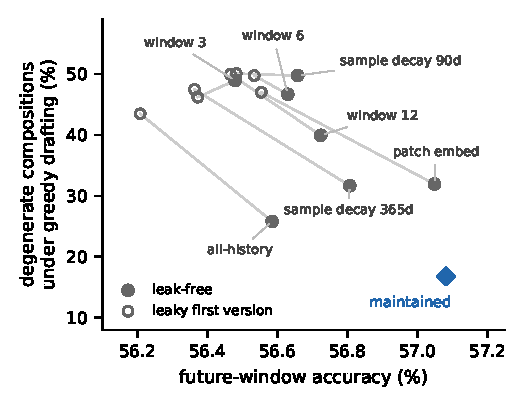
\includegraphics[width=\columnwidth]{fig_scatter.pdf}
\caption{Future-window accuracy against greedy degenerate-composition
rate for the eight training regimes, leak-free (filled) and in the
leaky first version (hollow, joined to their leak-free counterpart).
Removing the leak moves the all-history regimes down and to the right;
the short-history regimes stay degenerate.}
\label{fig:scatter}
\end{figure}

Leak-free, the regimes' future-window accuracies span 56.48\% to
57.08\%, 0.6pp. Their rates of broken teams under greedy drafting span
16.8\% to 49.7\%, a factor of three. Accuracy says little about which
regime is which. Across the seven cutoff-frozen regimes, the correlation
between future accuracy and degeneracy is $-0.46$ ($n = 7$, not
significant), and the patch-embedding regime, within 0.03pp of
\maintained{}'s accuracy, drafts broken teams at 31.9\% against 16.8\%
(Welch $t = 11.0$, 2.6 df, $p = 0.003$, three seeds each). Selecting
among these regimes by accuracy would call the best two
interchangeable.

History length accounts for most of the spread: regimes that see
mostly recent builds, by window or by 90-day sample decay, draft broken
teams 40\% to 50\% of the time, and regimes that keep all history sit at
26\% to 32\%. Training statistics aligned with each game's own era may
lower the rate further. With the opponent pool restricted to an
opponent model trained only to the cutoff, all-history training on
cutoff-frozen statistics drafts broken teams 23.3\% of the time against
14.1\% for \maintained{} (Welch $t = 7.0$, 2.6 df, $p = 0.01$); with the
earlier paper's opponent model, which saw the test period, the rates
are 25.8\% and 16.8\% ($t = 3.3$, 2.1 df, $p = 0.08$). Three seeds per
arm make these tests weak, seed spread is large in some cells (standard
deviation 4.7 points for all-history, 7.9 for the 12-build window), and
we do not detect the difference at the agent level
(Section~\ref{sec:neglect}).

Our first version reported a 2.5-fold gap (43.5\% against 16.8\%) and a
correlation of $+0.78$ between accuracy and degeneracy within the
standard regimes, which we read as accuracy ranking policies backwards.
The leak produced both (Figure~\ref{fig:scatter}). It raised the
degeneracy of the all-history regimes most (from 25.8\% to 43.5\%, 31.7\%
to 47.5\%, and 31.9\% to 47.0\%; Welch $t = 5.8$, 2.9 df, $p = 0.01$
for all history), moved the short-history regimes to 46\% to 50\%, and
lowered every regime's future accuracy by 0.1 to 0.5pp. What remains is
that at equal accuracy, policies can differ twofold in how often they
draft a broken team, so policy metrics have to be measured directly.

\section{What Retraining and Refresh Are Worth}
\label{sec:replay}

We replay a 2.8-year deployment forward across 36 builds, starting from
about 640{,}000 games of history at build 2.55.3.89754 (July 2023), and
score every maintenance policy by games-weighted accuracy and by regret
against retraining after every build (Table~\ref{tab:regret}). Every
maintenance-policy row trains on causal statistics with seed 42; the
frozen-statistics rows are the out-of-fold recipe (three seeds) and the
leaky construction (one seed). Differences between rows of a few
hundredths of a point are within the noise one training seed adds.

\begin{table}[t]
\caption{Deployment replay over 2.8 years: deployment-weighted regret
against retraining after every build, one training seed. ``Refresh''
recomputes statistics at every build; ``no refresh'' recomputes them
only at retrains. $^{a}$Three seeds.}
\label{tab:regret}
\centering
\footnotesize
\setlength{\tabcolsep}{3pt}
\begin{tabular}{lccc}
\toprule
Policy & Retrain & Refresh & Regret (pp) \\
\midrule
reference: retrain every build & 35 & 35 & 0.000 \\
\midrule
never retrain, never refresh & 0 & 0 & +1.021 \\
\quad frozen-statistics recipe, leak-free$^{a}$ & 0 & 0 & +1.01 to 1.35 \\
\quad frozen-statistics recipe, leaky & 0 & 0 & +1.698 \\
\midrule
never retrain, refresh every build & 0 & 35 & +0.662 \\
never retrain, refresh every 3rd & 0 & 11 & +0.685 \\
never retrain, 14 even refreshes & 0 & 14 & +0.675 \\
never retrain, detector refreshes & 0 & 14 & +0.677 \\
\midrule
retrain every 3, no refresh & 11 & 11 & +0.028 \\
retrain every 3, refresh & 11 & 35 & $-$0.002 \\
retrain every 6, no refresh & 5 & 5 & +0.146 \\
retrain every 6, refresh & 5 & 35 & +0.081 \\
finetune every 3, refresh & 11 & 35 & $-$0.005 \\
retrain every 9 / 12, refresh & 3 / 2 & 35 & +0.17 / 0.20 \\
\bottomrule
\end{tabular}
\end{table}

Doing nothing costs 1.02pp over the deployment. Refreshing the
statistics every build, with the weights fixed, recovers 0.36pp of it,
35\%. Retraining every three builds recovers 0.99pp even when the
statistics are recomputed only at each retrain, and refreshing between
retrains then adds 0.03pp; at a six-build cadence it adds 0.07pp.
Retraining does the repair. Refresh recovers a third of the loss when
retraining is impossible, and adds a few hundredths of a point once
retraining is scheduled. With refresh, cadences from one to six builds
land within 0.08pp of the reference, and the regret grows past that
(0.17pp at nine builds, 0.20pp at twelve). A warm-start finetune on the
last six builds matches a full retrain. In calendar terms the replay's
builds average 29 days apart, so a three-to-six-build cadence is
quarterly to twice a year.

Refresh does little on the future window of the main split too. Holding
the \maintained{} checkpoints fixed and freezing their statistics at the
cutoff lowers future-window accuracy by only 0.035pp (56.98\% to
56.95\%), a three-month horizon. The leak-free all-history model scores
56.68\%. So at the 2026 cutoff, 0.27 of the 0.30pp that separates the
two training recipes comes from training against statistics aligned with
each game's own era, and 0.035pp from refresh. In the replay the recipe
difference is within seed noise: the frozen-statistics recipe's three
seeds lose 1.01 to 1.35pp, bracketing the never-refreshed causal model's
1.02pp. The leaky construction puts the frozen-statistics recipe at
1.70pp.

\textbf{Decayed aggregates.} If recomputing statistics helps a little,
old games may deserve less weight inside them. Decaying the aggregates
exponentially, with the decay applied per build at each build's last
game date, raises future-window accuracy from 56.98\% (cumulative) to
57.17\% with a 90-day half-life, 57.23\% with a 90-day half-life and counts
shrunk toward the cumulative value (100 pseudo-games), and 57.18\% with a
365-day half-life. Paired on the same rows, with each arm's three seeds
averaged and standard errors clustered by game, the gains are +0.19pp
($z = 3.0$), +0.24pp ($z = 4.2$), and +0.20pp ($z = 4.2$). The half-life
itself is not identified. A nested check that repeats the selection at
an earlier cutoff and scores the four builds before the 2026 cutoff
finds no reliable difference from cumulative statistics ($-$0.02,
+0.03, and +0.06pp; $|z| \le 1.3$). We therefore recommend decaying the
aggregates without claiming a best half-life. Decaying each signal class
at its own measured rate does no better: hero-family statistics on a
90-day clock with pair and composition statistics on a 365-day clock
score 57.07\%, the reverse assignment 57.14\%.

\textbf{What refresh touches.} A partial-refresh ablation on the fixed
\maintained{} checkpoints swaps statistics by signal class at test time.
Every effect is within $\pm$0.07pp over the three-month horizon.
Refreshing hero-level statistics alone lowers accuracy by 0.02pp;
refreshing pair and composition statistics alone raises it by 0.07pp,
more than refreshing everything (+0.035pp). Raw pair win rates drift as
fast as hero win rates, and the pair features are normalized by hero
win rates, so the pair-only cell also carries current hero strength,
and the hero-only cell feeds the model mismatched numerators and
denominators; we draw no conclusion about which signal class matters.

\section{The Cost of Neglect, Head-to-Head}
\label{sec:neglect}

Accuracy comparisons leave open whether any of this matters when
policies play. We answer with direct competition. Two agents draft
against each other in every pairing of their seeds, both first-pick
orderings, 40 drafts per ordering (10 for the 15$\times$15 first-version
matchups) over stratified maps and tiers, each
agent acting greedily from its policy head. At play time no agent uses
aggregate statistics; statistics enter only through the value function
and the kernel's statistics table during MCTS training. ``Maintenance''
at the agent level therefore means a policy trained against refreshed
statistics, which is a retrain.

The agents share one MCTS recipe (200 simulations, 300{,}000
self-play episodes) and differ in their value function, the statistics
table used during training, and the opponent model. \maintained{} is our
earlier agent, 15 MCTS seeds; its value function is the one of three
\maintained{} seeds with the best future-window accuracy, a selection
worth at most 0.07pp of accuracy. A replication of \maintained{} with
6 MCTS seeds, two on each of the three value-function seeds, charges
value-function variance. \stalefour{} has 6 MCTS seeds, two on each of
three leak-free value-function seeds. \mcut{} holds \maintained{}'s
selected value function and trains its policy on statistics frozen at
the cutoff (5 seeds); it is the maintained recipe trained at the cutoff
and then left alone. \staleone{} and \staletwo{} use the leak-free value
functions trained to their own cutoffs, statistics of that date, and an
opponent model trained only on games up to that date, for both the
policy's initialization and its self-play opponent (3 and 6 seeds; the
one-year arm was cut to one agent per value-function seed when compute
was capped). The 2026 agents are initialized from, and trained against,
the earlier paper's opponent model, which saw the test period, so both
sides of every 2026 matchup share it. To compare staleness with the
opponent model matched by era on both sides, we also trained
\stalefour{} against an opponent model fit only to games before the 2026
cutoff (U-era below, 4 seeds).

Each terminal draft is scored against the realized outcomes of later
games: the average win rate of the heroes each side picked, the synergy
of each side's pairs and its counters against the other side (pair and
matchup win rates beyond what the heroes' own rates predict), and the
rule-based degenerate-composition flag. The scoring games are the
298{,}428 ranked games of build 2.55.16.97039 and the four 2.55.17
builds (May through September 2026). No agent's statistics include
them. The first 12{,}337 games of 2.55.16.97039 fell inside the pinned
future window, which we used to select value-function seeds and the
decay half-life and which trained the earlier paper's opponent model;
on the 150{,}131 games of the four 2.55.17 builds alone, which no part
of any agent saw, every contrast below keeps its sign and size (for
example $+0.46$pp for \maintained{} against \stalefour{}, $p = 0.007$).
Our first version of this protocol scored against all seven post-cutoff
builds, six of which also fed \maintained{}'s statistics; that overlap
tripled the synergy gap. Inference uses crossed random effects for the
two seed identities with a $t$ reference and Satterthwaite degrees of
freedom. The primary contrast is future-meta hero win rate; synergy,
counters, degeneracy, and the other truth sets are secondary.

\begin{table}[t]
\caption{Head-to-head results on out-of-sample builds. $\Delta$: the
first agent's advantage in future-meta hero win rate (pp, crossed seed
random effects, $t$ reference). Net: team win-probability gap from a
realized-outcome index with hero, synergy, counter, and
role-composition terms and three structure indicators (no healer, no
frontline, stacked role), weights fitted on held-out real games (two
cross-fitting folds); it uses the 308{,}375 games of the same five
builds that our database held on September 29, 2026, dated no later
than September 27. M: \maintained{}; M-d90: \maintainedpred{}; M-cut:
\mcut{}; U: \stalefour{}; U-era: \stalefour{} with a cutoff-era opponent
model; S1, S2: \staleone{}, \staletwo{}; M-vol: \maintained{} trained on
S2's row count; U-leaky, S2-leaky: the leaky first versions.}
\label{tab:dose}
\centering
\footnotesize
\setlength{\tabcolsep}{3.5pt}
\begin{tabular}{lcccc}
\toprule
Matchup & Seeds & $\Delta$ (pp) & $t$ (df) & Net (pp) \\
\midrule
\multicolumn{5}{l}{\emph{same cutoff}} \\
M (all VF seeds) vs U & 6$\times$6 & $+0.34 \pm 0.17$ & 2.0 (10) & +1.5 \\
M vs U & 15$\times$6 & $+0.43 \pm 0.13$ & 3.3 (10) & +2.7 \\
M-d90 vs U & 15$\times$6 & $+0.77 \pm 0.11$ & 7.0 (8) & +3.4 \\
M vs M-cut & 15$\times$5 & $-0.05 \pm 0.11$ & $-0.5$ (9) & $-0.6$ \\
M-cut vs U & 5$\times$6 & $+0.52 \pm 0.13$ & 3.9 (10) & +3.3 \\
U vs U-era & 6$\times$4 & $+0.24 \pm 0.21$ & 1.1 (8) & +0.6 \\
\multicolumn{5}{l}{\emph{staleness, era-matched opponent models}} \\
U-era vs S1 & 4$\times$3 & $+0.97 \pm 0.15$ & 6.4 (3) & +5.7 \\
U-era vs S2 & 4$\times$6 & $+0.64 \pm 0.14$ & 4.8 (8) & +2.5 \\
\multicolumn{5}{l}{\emph{staleness, 2026 side on the earlier paper's opponent model}} \\
U vs S1 & 6$\times$3 & $+1.12 \pm 0.23$ & 4.8 (5) & +5.2 \\
U vs S2 & 6$\times$6 & $+1.00 \pm 0.16$ & 6.3 (8) & +3.4 \\
M vs S1 & 15$\times$3 & $+1.34 \pm 0.16$ & 8.6 (3) & +6.7 \\
M (all VF seeds) vs S2 & 6$\times$6 & $+1.28 \pm 0.15$ & 8.7 (9) & +4.6 \\
M vs S2 & 15$\times$6 & $+1.40 \pm 0.09$ & 15.9 (13) & +6.1 \\
M-vol vs S2 & 5$\times$6 & $+1.28 \pm 0.16$ & 8.1 (7) & +6.2 \\
\multicolumn{5}{l}{\emph{leaky controls (first version)}} \\
M vs U-leaky & 15$\times$15 & $+0.69 \pm 0.10$ & 7.0 (32) & +3.3 \\
M vs S2-leaky & 5$\times$5 & $+1.10 \pm 0.17$ & 6.5 (8) & +4.5 \\
U vs U-leaky & 6$\times$15 & $+0.35 \pm 0.13$ & 2.8 (11) & +1.9 \\
\bottomrule
\end{tabular}
\end{table}

Against the leak-free unmaintained agent, the maintained agent's 15
seeds average +0.43pp of future-meta hero win rate ($t = 3.3$, 10 df,
$p = 0.008$; Table~\ref{tab:dose}), about 2.7 points of team win
probability by the realized-outcome index, and the advantage holds on
both halves of the scoring set (+0.41pp on 2.55.16.97039, +0.46pp on
the 2.55.17 builds). Those 15 agents share one value function, so this
estimate conditions on one value-function draw. The replication that
varies the value-function seed gives $+0.34 \pm 0.17$pp ($t = 2.0$,
10 df, $p = 0.07$). Its six agents range from $-0.12$ to $+0.82$pp, and
the 15 single-value-function agents from $-0.01$ to $+0.93$pp, so
agent-seed variance dominates at this effect size; averaged by
value-function seed the replication gives $+0.35$, $+0.38$, and
$+0.30$pp, so no single value function carries it. We read the
same-cutoff advantage as about a third of a point, positive in every
estimate and significant only with the larger seed budget. Our first
version measured +0.66pp against the leaky agent (+0.69pp at fifteen
seeds per side), so between a third and a half of the advantage we
first reported came from the leak; the two unmaintained agents compared
directly differ by +0.35pp ($t = 2.8$), and the leak-free one drafts
broken teams 28\% of the time against 50\%. The decayed-statistics
agent leads the unmaintained agent by +0.77pp ($t = 7.0$), consistent
with its lead over \maintained{} in Section~\ref{sec:replay}.

The leak also produced two claims we retract. The first version found
that unmaintained agents counter the maintained agent's picks slightly
better ($-0.31 \pm 0.08$ in counter score at fifteen seeds). Against the
leak-free agent the sign flips and the gap is small ($+0.12 \pm 0.07$ for
\maintained{}, $t = 1.7$), and the leak-free agent counters worse than the
leaky one ($-0.39 \pm 0.09$, $t = -4.3$). The first version also found
that maintenance cut broken teams from 36.9\% to 22.0\% in head-to-head
play. Against the leak-free agent the rates are 24.1\% and 29.7\%
($-5.6 \pm 7.6$ points, not significant). At the agent level we cannot
detect a degeneracy benefit from maintenance, although the greedy
protocol of Table~\ref{tab:regimes} suggests one. Synergy differences
are small in every same-cutoff matchup ($+0.14 \pm 0.11$ here).

The \mcut{} agent locates the advantage. It keeps \maintained{}'s
selected value function and trains its policy on statistics frozen at
the cutoff. Against \maintained{}, whose policy trained on three more
months of statistics, it is level ($-0.05 \pm 0.11$pp, 95\% interval
$-0.30$ to $+0.19$). Against \stalefour{}, which differs from it in how
its value function's training statistics were built, it leads by
$+0.52 \pm 0.13$pp ($t = 3.9$). This is consistent with the advantage
coming from training the value function on statistics aligned with
each game's era, with three months of refresh adding little: the
interval excludes refresh effects larger than about 0.2pp, matching the
0.03pp refresh adds on the accuracy side (Section~\ref{sec:replay}).
Both \mcut{} and \maintained{} use one selected value function, so this
split conditions on that draw. The first row of Table~\ref{tab:dose}
therefore compares training recipes: an agent trained once at the
cutoff with the causal recipe already has the advantage. The cost of
neglect proper is the gap between agents built with the same recipe at
different cutoffs.

Staleness costs more than the same-cutoff gap, by an amount that depends
on how the comparison treats the opponent model. With era-matched
opponent models on both sides (U-era against \staleone{} and
\staletwo{}), the agent trained at the 2026 cutoff leads the one-year
agent by $+0.97 \pm 0.15$pp ($t = 6.4$, 3 df) and the two-year agent by
$+0.64 \pm 0.14$pp ($t = 4.8$, 8 df), about 2.5 to 6 points of team win
probability (Figure~\ref{fig:dose}). The one- and two-year gaps cannot be
told apart, so we make no claim about when within the first two years
the loss arrives. When the 2026 side keeps the earlier paper's opponent
model, which saw the test period, the gaps grow to $+1.12$ and
$+1.00$pp, and against \maintained{} to $+1.34$ and $+1.40$pp ($+1.28$
with value-function seeds varied); the opponent model alone is worth
$+0.24 \pm 0.21$pp to the 2026 agent (not significant). So part of the
gap in those rows is the opponent model, and the era-matched rows are
the cleaner estimate of staleness. Because our corpus grows over time,
the two-year agent also trained on fewer games; a maintained agent
trained on \staletwo{}'s row count keeps $+1.28$pp, 91\% of its gap.

The interaction metrics also depend on the opponent model. With
era-matched opponents, the stale agents show no synergy deficit
($-0.06 \pm 0.08$ at two years, $-0.17 \pm 0.07$ at one) and counter
worse than the 2026 agent ($+0.27 \pm 0.12$ for U-era at two years).
With the 2026 side on the earlier paper's opponent model, the two-year
agent shows a synergy deficit ($+0.21 \pm 0.08$ against \maintained{})
and no counter difference. The first version's ``synergy does not rot''
and ``the stale agent counters better'' came from agents that shared the
earlier paper's opponent model and a leaky value function; with the
leak removed and the opponent models matched, synergy shows no
staleness cost and counters favor the newer agent. The leaky first
version put the one-year gap at $+0.56 \pm 0.21$pp.

\begin{figure}[t]
\centering
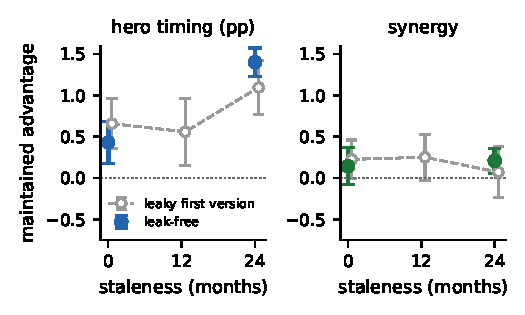
\includegraphics[width=\columnwidth]{fig_dose.pdf}
\caption{Cost of staleness in future-meta hero win rate (left, pp) and
synergy (right), scored on out-of-sample builds, with 95\% $t$ intervals
from crossed seed random effects. The agent trained at the 2026 cutoff
(0 months, the reference) against leak-free agents trained one and two
years earlier. Filled: opponent models matched by era on both sides
(U-era against S1, S2). Hollow: the 2026 agent on the earlier paper's
opponent model, which saw the test period (U against S1, S2).}
\label{fig:dose}
\end{figure}

\section{What Drifts}
\label{sec:signals}

Per-build statistics let us measure how each signal class decays.
Correcting each correlation for binomial sampling noise (disattenuated
$r$), role-composition win rates are nearly static, at 0.95 with
themselves over a lag of 16 builds. Hero pick rates are nearly as stable
(0.89 at lag 16). Per-hero win rate is the fastest-decaying reliable
signal, falling from 0.94 at lag 1 to 0.62 at lag 16 (raw correlations
0.85 and 0.57). Raw pair win rates track their component hero win rates
(0.61 at lag 16; Figure~\ref{fig:decay}). The pairwise interaction
beyond the two heroes' strengths is weak and mostly within-build
sampling noise, a caution for pairwise features generally. The value
model ages as well. Scored on the same rows, the seven builds after the
2026 cutoff, each with its own frozen statistics, the leak-free
all-history model trained at the 2026 cutoff has calibration slope 0.96,
and models trained one and two years earlier have 0.79 and 0.75 (three
seeds each; seed ranges 0.93 to 0.99, 0.78 to 0.80, and 0.72 to 0.77).

\begin{figure}[t]
\centering
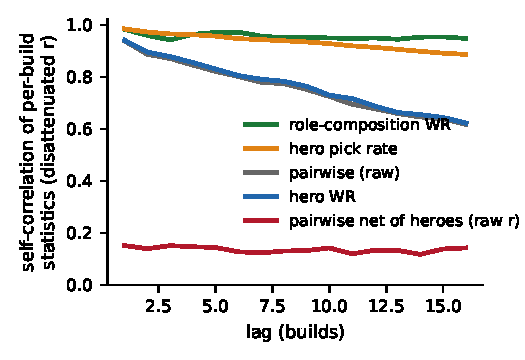
\includegraphics[width=\columnwidth]{fig_decay.pdf}
\caption{Signal-class decay: self-correlation of per-build aggregate
statistics against build lag, corrected for binomial sampling noise
(disattenuated $r$), except the net pairwise series, which shows raw
$r$ because its reliability is near zero.}
\label{fig:decay}
\end{figure}

Two questions a maintainer asks after every patch have answers here.
First, how soon can a new build's own statistics be trusted? Measured
against the build's remaining games, which is what a deployed system can
check, patch-local hero win rates come within a point of the truth after
a median of about 17{,}100 games into a build. (A popular alternative,
distance to the build's final value, reaches the same threshold at
10{,}800 games, but the early games are part of the final value, and its
error matches pure sampling error at every checkpoint, so it measures
accumulation more than settling.) At the snapshot's early-2026 rate of
about 11{,}000 ranked games per week that is about a week and a half,
and at the 14{,}000 to 16{,}000 per week we measured for the
pre-registration, about eight days. Second,
does drift change which compositions never get played? The observed
composition sets of consecutive builds have a mean Jaccard similarity of
0.81, and the per-build never-fielded count follows build volume
($r = -0.98$ against log games). Built from each era's history, the
never-fielded targets of our earlier paper's synthetic-augmentation
method stay within 24 compositions per tier of the full-corpus target
from about three years of history on, and within 2 at the cutoff; the
earliest eras differ by up to 99.

\section{Detecting Balance Changes from Outcomes}
\label{sec:detect}

A maintainer wants to know when the game changed. The developer's patch
notes provide ground truth: we scripted 40 mapped patches, and five
builds have no published notes and count as no-change builds. The
detector tests each hero's win rate across each boundary between sizable
builds (two-proportion test, at least 200 games per side) and keeps the
shifts that survive Benjamini--Hochberg correction at $q = 0.05$ within
the boundary. A boundary fires when at least one hero survives.

The ground truth has two variants, and we report both. The scripted
truth counts every hero the notes mention, including heroes mentioned
only for bug fixes; this is what the frozen detection code uses. A
balance-only variant drops bug-fix-only mentions, which appear in 22 of
the 40 mapped patches (458 mentions). At the hero level, 46 of the detector's 59
flags name a hero the notes mention (0.78), and 39 of 59 name a hero with
a balance change (0.66). A randomly chosen hero at a random boundary is
mentioned about 30\% of the time. At the boundary level, the detector
fires on 16 of the 21 boundaries whose notes mention a hero and on 1 of
the 6 without (one-sided Fisher exact $p = 0.015$); under the
balance-only truth, 15 of 19 against 2 of 8 ($p = 0.014$). Boundary
precision, 16 of 17, sounds stronger than it is, because 21 of 27
boundaries carry mentions and random firing would already score 0.78
(binomial $p = 0.08$). The controls are few, and five of the six
no-change boundaries fall inside one maintenance era (2.55.3).
Two misses are roster-wide cleanup patches that mention 88 and 64 heroes;
at 2.55.2.88122 all three flags fall outside the notes. Per-hero recall
is low (0.06), because the notes list every individual change and most
are too small to detect singly. The same test on pick and ban rates has
hero-level recall 0.69 and precision 0.32; it picks up the community
reacting, which spills across build boundaries and fires on hype as
readily as on tuning.

How fast does it know? The first flagged hero at each firing boundary
crosses an uncorrected $p < 0.05$ threshold a median of 2{,}500 games
into the build. Over all 46 true-positive flags, the uncorrected first
crossing has median 6{,}900 games. A Bonferroni-corrected sequential
test never flags 7 of the 46 before the build ends, and flags the other
39 after a median of 18{,}800 games. The detector's fire decisions themselves use the
full build.

As a refresh trigger the detector performs like a calendar. In the
replay of Table~\ref{tab:regret}, refreshing a fixed model only when the
detector fires gives +0.677pp regret, against +0.675 for 14 evenly
spaced blind refreshes, +0.685 for a refresh every third build, and
+0.662 for every build; the differences are within the replay's noise.
The detector arm is a hindsight upper
bound: which boundaries fire is decided with the full build and with the
sizable-build list known in advance, and each refresh is then placed at
the first-detection time of a hero the full-build test flags. Latency
itself costs 0.003pp; the sparser schedule costs 0.012pp.
Recomputing statistics is cheap, so saving refreshes has little value.
Sweeping the false-discovery level across two orders of magnitude moves
hero-level precision from 0.90 (17 of 19 flags) to 0.44, and every
operating point lands within 0.05pp of every other on the replay. Of the
replay's 36 builds, 20 are sizable; the detector fires on 14 of the 20
boundaries ending at them, one of which (2.55.10.94470) has no
documented change.

The detector's value is as an alarm, and it needs little. It uses
version identifiers, which almost every deployed system logs, and the
magnitude of the outcome shift between versions; it needs no patch
notes or labels. We also tested whether change timing could be recovered
without version identifiers: a multi-scale changepoint detector over
daily hero pick, ban, and win rates, tuned on pre-2025 boundaries (its
best family was pick and ban rates), reaches held-out precision 0.18 at
recall 0.27. With a $\pm$3-day tolerance, the 11 held-out boundaries
cover about 77 of the 507 held-out days, so chance precision is about
0.15. Without
version identifiers we could not reconstruct the change calendar.

\section{Evaluators Drift Too}
\label{sec:vintage}

The obvious way to score the head-to-heads was the consensus of our
win-probability models, the panel that adjudicated our earlier
tournament. We did that first, got +0.8pp for the maintained side, and
then noticed the number was unidentified: those judges were trained on a
snapshot that includes the future period, so they share the maintained
agent's information advantage by construction. The fix produced a
finding about judges.

We trained naive-feature judges (hero identities, map, and tier; no
aggregate statistics) in two corpus families and scored the 7{,}200
drafts of the \maintained{} versus \stalefour{} head-to-head of
Section~\ref{sec:neglect} with every judge, and also the 2{,}000 drafts
of our first head-to-head against \leakyunm{}. Here the drafts are a
test set; the question is how judges of different eras score the same
drafts, against a realized-outcome verdict that favors the maintained
side. Six
ranked-play judges span early 2022 through the cutoff, each trained on
the 314{,}761 most recent games before its cutoff (158{,}709 for the
earliest, 2022Q1). These judges' training data are subsets of both
agents' training data, and the 2026 judge's window ends at the cutoff.
Four Quick-Match judges (2021, 2022, 2024, 2026, on pools of 29K to
129K games) come from a mode with no draft phase: the matchmaker
assembles teams, so these judges never saw a draft.

On the leak-free drafts the ranked verdict rises with judge era: 0.462
(2022Q1) and 0.479 (2022-07), 0.487 (2023), 0.488 (2024), 0.512 (2025),
and 0.525 (2026). The Quick-Match family repeats the pattern: 0.428
(December 2021) and 0.432 (2022), then 0.487 (2024) and 0.522 (2026).
Each score has two sources of error: draft sampling, which we estimate
with standard errors clustered by seed pairing (0.002 to 0.008), and the
judge's own training seed, whose standard deviation is up to 0.011 (range
up to 0.021 across the three seeds of the 2026 ranked judge). Combining
the two in quadrature, every judge trained before 2023 declares the
unmaintained agent the winner of a 2026 contest, by 1.9 to 5.4 combined
standard errors; the 2023 and 2024 judges lean the same way by about one;
the 2025 and 2026 judges side with the realized outcome, by 1.1 to 2.1.
The first-version drafts give the same picture (pre-2023 judges 0.416
to 0.469, later judges 0.493 to 0.508). The 2026 Quick-Match pool has no
upper date bound, and 32\% of its games postdate the cutoff; retrained
with the pool capped at the cutoff, it scores the first-version drafts
\capqm{} over three seeds, so the verdict does not change. Because the
Quick-Match family moves from about 0.43 to 0.52 with the game mode
fixed, the reversal tracks the judge's era within one corpus family
(Figure~\ref{fig:vintage}).

\begin{figure}[t]
\centering
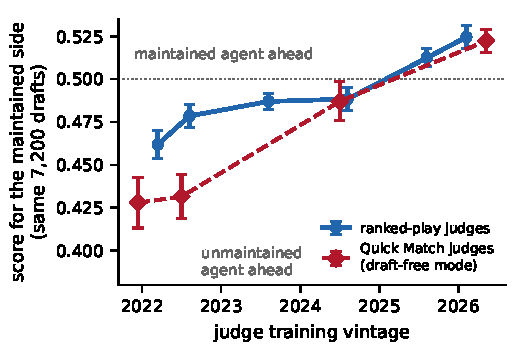
\includegraphics[width=\columnwidth]{fig_vintage.pdf}
\caption{The vintage matrix. Score assigned to the maintained side of
the 7{,}200 leak-free \maintained{} versus \stalefour{} drafts by
win-probability judges trained at different times (95\% intervals,
normal approximation, clustered by seed pairing; judge-seed variation is
not included). Realized outcomes favor the maintained side. Judges
trained before 2023 reverse the verdict, and judges from 2025 on agree
with it. Diamonds: judges trained on Quick Match, a mode without a
draft phase.}
\label{fig:vintage}
\end{figure}

The oldest and newest Quick-Match judges (December 2021 and 2026) both
reproduce our earlier tournament's ordering of 11 strategies at rank
correlation 0.90. Contests decided by composition structure are stable
across eras, because structure barely drifts
(Section~\ref{sec:signals}); contests decided by meta timing are where
judge vintage matters. Anyone evaluating agents in a drifting domain
should date each judge and report the judge-by-era matrix, with the
headline on realized outcomes.

\section{The Opponent Model Drifts on Its Own Clock}
\label{sec:opponent}

A deployed drafter also carries a behavioral model of its opponent (the
next-pick predictor that guides search), and player behavior drifts on a
different schedule than balance. We compared opponent models on 1.84
million next-pick samples from the future builds
(Table~\ref{tab:gdpools}).

\begin{table}[t]
\caption{Opponent models scored on 1.84M future next-pick samples
(top-1/top-5 accuracy, \%). Rows 1 and 4 saw the test drafts in
training and are references only. $^{a}$Retrained before each test
build on the preceding 30 days of play.}
\label{tab:gdpools}
\centering
\small
\setlength{\tabcolsep}{4pt}
\begin{tabular}{lcc}
\toprule
Model (training data) & Top-1 & Top-5 \\
\midrule
test-period fit (98\% of the test drafts) & 13.09 & 40.39 \\
30 days before each build (rolling)$^{a}$ & \textbf{11.97} & -- \\
30 days before the cutoff, trained once & 11.83 & \textbf{36.98} \\
earlier paper's model (full snapshot) & 11.71 & 36.31 \\
last 6 builds before the cutoff & 11.64 & 36.91 \\
all history to the cutoff & 11.08 & 34.47 \\
\bottomrule
\end{tabular}
\end{table}

With the same two model variants in each row, the earlier paper's model
scores 11.76\% top-1, 0.68pp above the all-history model deployable at
the cutoff; that is a lower bound on behavioral drift, since only about
7\% of the earlier model's training data postdates the cutoff. Recency
recovers most of the gap: a model trained on the last six builds gains
0.56pp, and one trained once on the 30 days before the cutoff gains
0.75pp, finishing 0.08pp above the earlier paper's model. The 30-day
model's lead fades. It is the best model on the three 2.55.15 builds
(13.1\%, 12.6\%, and 12.2\% top-1) and beats the all-history model on the
first two 2.55.16 builds, but it is the worst model on the last two,
falling to 10.6\% against 11.2\% for the all-history model. It wins on
bans (17.1\% against 16.2\%) and loses on picks. Rolled forward,
retraining on the 30 days before each build, the window scores 11.97\%
overall, 0.14pp above the once-trained model and 0.89pp above the
all-history model, and 11.5\% on the last build instead of 10.6\%. It
trails the all-history model on one build (2.55.16.96881, 10.7\% against
11.0\%). Behavior favors a rolling window, retrained often.

Before running this comparison we set a rule for escalating it: retrain
the MCTS pipeline on refreshed opponents if behavioral drift cost at
least 1.0pp of top-1, or if swapping opponent pools moved the maintained
value function's greedy healer or degeneracy rates by at least 3pp. The
rule lives in our analysis code, dated by file timestamps, and was not
publicly registered. Neither condition was met: 0.63pp of top-1, and
movements of 2.9pp in healer rate and 2.7pp in degeneracy (paired seed
standard errors 1.2 and 0.9pp, so the degeneracy movement missed the
threshold by 0.3pp at about 2.9 standard errors). The rule's accuracy
measure is the lower bound above; the rolling window's 0.89pp gain over
the all-history model, a less understated measure, also falls short of
1.0pp. The all-history
value function, which the rule did not cover, moved more (5.8pp of healer
rate, 3.5pp of degeneracy). By rule, the escalation did not run. For the
two stale agents we did train era-matched opponent models, because an
agent's counter-play is learned from its opponent
(Section~\ref{sec:neglect}).

\section{The Operating Policy}
\label{sec:operating}

The measurements above reduce to a short policy. Train on causal or
out-of-fold statistics and check calibration on rows the statistics
never contained. Retrain the value model on a fixed schedule; every
three to six builds (quarterly to twice yearly here) keeps regret within
about 0.1pp of retraining constantly. Recompute the statistics at each
retrain, and between retrains if it is free, which buys a few hundredths
of a point. Prefer 90-day decayed statistics. Retrain the opponent model
on recent play. Use the outcome-shift detector as an alarm that a
build changed hero strength; do not use it to schedule refreshes.

Our production deployment retrains all three models monthly on the full
corpus, with 90-day decayed statistics computed out of fold for training
rows, and serves the same decayed statistics to the browser; a
calibration-slope gate blocks deployment when the value model's slope on
held-out rows leaves [0.8, 1.25]. The first full run of this pipeline
completed and deployed on September 30, 2026 (slope 1.05); scheduled
monthly runs begin November 1, 2026. Builds have averaged about a month
apart, so a monthly retrain is close to retraining after every build,
more often than the replay says is necessary.\footnote{\deployurl}

\section{A Prospective Test, Pre-Registered}
\label{sec:prospective}

Every result above is retrospective: the cutoff was chosen, then the
future window was scored. So before submission we registered three
forward claims on OSF (\preregdate{}; \prereglink{}), with the analysis
code frozen by commit hash: (1) the outcome-shift detector, decision
rule untouched, fires on new builds whose patch notes contain hero
changes and stays silent on no-change builds (builds whose changes are
all individually minor are reported descriptively and adjudicate
nothing); (2) the existing 4{,}500-draft head-to-head between \maintained{}
and \leakyunm{}, rescored with the out-of-sample protocol of
Section~\ref{sec:neglect} against the new builds' realized statistics,
keeps a positive maintained advantage in future-meta hero win rate
(both agents and all drafts predate those builds, so nothing in this
claim can be tuned). The registered rule for C2 is a normal-reference
test of the crossed-random-effects estimate: confirmed if
$z \geq 1.645$ (one-sided $\alpha = 0.05$), falsified if the estimate is
at most 0, otherwise inconclusive. (3) Every production refresh event is logged and reported
against the detector's fires. The claims cover only builds that ship
after the registration date. The builds between our snapshot and the
registration (2.55.16.97039 and the four 2.55.17 builds) already serve as
the scoring set of Section~\ref{sec:neglect} and are excluded. The
analysis date is fixed at submission: \analysisdate{}. New ranked games
arrived at 14{,}000 to 16{,}000 per week when we registered, so a new
build reaches the 20{,}000-game detector gate in under two weeks, and a
six-month window should contain three or four sizable builds. The first
logged production refresh under C3 is the September 30, 2026 deployment
(Section~\ref{sec:operating}).

Three disclosures bear on the registered claims and will be repeated
when they are reported. The registration text says bug-fix-only and ARAM-only
hero mentions are excluded from the ground truth, as in the
retrospective analysis. The frozen code does not exclude them: it counts
every hero the notes mention. The registered test is the frozen code, so
C1 will be adjudicated with the any-mention truth, and we will also
report the balance-only variant. The retrospective numbers in
Section~\ref{sec:detect} report both. Second, the registered
head-to-head (C2) was drafted by \leakyunm{}, the leaky first version of
the unmaintained agent, because it was registered before the leak was
found. We will report it as registered and report the leak-free
matchups of Section~\ref{sec:neglect} alongside it as descriptive
results. Third, on September 30, 2026 our database relabeled skill tiers
into a new scheme (Section~\ref{sec:setting}), while the registered
drafts carry the snapshot's labels. The frozen truth-scoring code groups
games by the database label, so a rerun would score drafts against
statistics from a different tier grouping. We will reconstruct the
snapshot-scheme label from each game's stored league tier before
scoring, and report this as a deviation.
% [PROSPECTIVE RESULTS: filled at the revision analysis date, per
% paper/drift/PREREG_FORWARD.md. Submission does NOT wait for this
% section's results.]

\section{Related Work}
\label{sec:related}

Concept drift and dataset shift have a large literature, most of it
classifier-centric: detect distributional change, adapt the model,
measure accuracy~\cite{quinonero2009dataset,gama2014survey,lu2018learning}.
The canonical detectors monitor a supervised error stream (DDM tracks
error-rate inflation~\cite{gama2004ddm}; ADWIN maintains adaptive
windows over it~\cite{bifet2007adwin}), and adaptation means retraining
or reweighting the classifier. Change-point detection supplies the
standard machinery~\cite{aminikhanghahi2017survey}; our detector is
deliberately plain, and what we add is the ground truth we score it
against (developer patch notes) and its price as a maintenance trigger.
Our results sit on the retraining side of that literature: in this
domain, retraining on a schedule does almost all of the repair, and the
policy-level cost of drift is larger than the accuracy cost suggests.
Target leakage through aggregate statistics is a known failure in
tabular learning~\cite{kaufman2012leakage}, and ordered or out-of-fold
target statistics are the standard remedy~\cite{prokhorenkova2018catboost};
we show how it distorts a drift study specifically, by making the
unmaintained baseline look worse than drift does.

Continual and non-stationary reinforcement learning study policies that
keep learning as the environment changes~\cite{padakandla2021survey,
khetarpal2022continual}, with catastrophic forgetting as a central
obstacle~\cite{kirkpatrick2017ewc}. The deployed case we study fixes the
policy between maintenance events and asks when and what to touch; a
continual learner would still need a trigger and leak-free statistics. OpenAI Five kept one
Dota 2 agent current across game patches by ``surgery'' on its network
and continued training~\cite{berner2019dota}, a retraining-side answer
to the same problem at far larger scale. On the operations side, data
dependencies and feature freshness are a known maintenance surface of
deployed ML~\cite{sculley2015debt}, production-readiness rubrics score
monitoring loops~\cite{breck2017mltest}, data-validation systems treat
stale statistics as a failure~\cite{polyzotis2019data}, and practitioners
report retraining cadence as an open question~\cite{shankar2022operationalizing};
we supply a measured decomposition of what refresh and retraining each
buy in one domain.

In games, drafting has been treated as prediction and recommendation,
from pick prediction in Dota 2~\cite{summerville2016draft} to team-aware
hero recommendation~\cite{chen2018art} and personalized draft
recommendation~\cite{draftrec}. In this journal, Chen et al.\ learn to
draft with neural networks and MCTS~\cite{chen2021juewudraft}, and
Gourdeau and Archambault select heroes in professional Heroes of the
Storm and Dota 2 drafts with a discriminative network~\cite{gourdeau2021discriminative}.
Balance evaluation has its own methods~\cite{jaffe2012balance}. To our
knowledge none of this work measures maintenance policies against
patch-note ground truth or prices staleness in head-to-head play.
Offline reinforcement learning under non-stationarity is usually posed
as a training-time problem~\cite{levine2020offline}; here the policy is
fixed and the world moves. This paper is the time-axis companion to our
draft-policy paper~\cite{paper1}. Player-skill drift is out of scope and
is the subject of a companion study of personalization.

\section{Limitations}
\label{sec:limits}

Everything here is one game and one major patch, a scoping that buys 45
builds with a fixed hero pool at the cost of external validity. The
deployment replay uses one training seed per cell; orderings among
regrets from different models within about 0.07pp (for example 0.050
and 0.067) are at noise level, although paired comparisons on the same
models, such as refresh against no refresh at a fixed cadence, are
not. The judge-free protocol
rests on realized hero, pair, and matchup statistics, which are
marginal quantities; we mitigate by triangulating the metrics and by
combining them with weights fitted on held-out real games.
Agent-level comparisons carry several caveats. Except for U-era, the
2026 agents share the earlier paper's opponent model, which saw the test
period; the era-matched staleness rows rest on 4 U-era seeds. Seed budgets changed
during the work: the maintained replication was scored at 3 and 5 seeds
before reaching its planned 6, and the one-year arm was cut from 6 seeds
to 3. \maintained{}'s value function was
selected on the future window from three seeds, and \mcut{} shares it,
so the split between them conditions on one value-function draw; with
value-function seeds varied, the same-cutoff advantage is not significant
($p = 0.07$). The leak-free staleness
gradient's one-year point rests on three agent seeds. We tested about
twenty accuracy cells on the same future window and many
matchup-by-metric combinations; we name the primary contrasts in each
section and treat the rest as secondary. Finally, our analysis went
wrong three times before this version: an evaluator panel that shared the
maintained agent's vintage (Section~\ref{sec:vintage}), scoring games
that overlapped the maintained agent's statistics
(Section~\ref{sec:neglect}), and unmaintained baselines trained on their
own outcomes (Section~\ref{sec:setting}). The last one changed the
paper's main conclusion, and we cannot rule out further errors of the
same kind.

\section{Conclusion}

A draft policy that nobody maintains loses about a point of accuracy
over three years of balance changes. Retraining on a schedule of three
to six builds recovers nearly all of it; refreshing statistics with the
weights fixed recovers a third, and adds a few hundredths of a point
once retraining happens. At the agent level, three months without
refresh cost nothing measurable, and one or two years cost two thirds
of a point to a point of future-meta hero win rate. Accuracy
understates the policy-level damage, and learned judges are as
era-bound as the models they score.

\ifanonymous
\section*{AI Disclosure}
Portions of this manuscript's text were drafted and edited with Claude
(Anthropic)~\cite{claude}; the authors designed and verified all
experiments and approved the text.
\else
\section*{Acknowledgments}
We thank Heroes Profile for API access to replay data (a paid service,
and an open-source project we are glad to support), and the NGS
community for organized-league data used in our earlier work. Portions
of this manuscript's text were drafted and edited with Claude
(Anthropic)~\cite{claude}; the authors designed and verified all
experiments and approved the text.
\fi

\begin{thebibliography}{99}
\bibitem{paper1} \ifanonymous Anonymous authors\else M.~Segan,
E.~Pysher, J.~Frankel, and H.~Lipson\fi, ``Diagnosing and repairing
out-of-distribution failure in MOBA draft policies,'' under review,
2026.
\bibitem{quinonero2009dataset} J.~Qui\~nonero-Candela, M.~Sugiyama,
A.~Schwaighofer, and N.~D. Lawrence, Eds., \emph{Dataset Shift in
Machine Learning}. MIT Press, 2009.
\bibitem{gama2014survey} J.~Gama, I.~\v{Z}liobait\.{e}, A.~Bifet,
M.~Pechenizkiy, and A.~Bouchachia, ``A survey on concept drift
adaptation,'' \emph{ACM Computing Surveys}, vol.~46, no.~4, 2014.
\bibitem{lu2018learning} J.~Lu, A.~Liu, F.~Dong, F.~Gu, J.~Gama, and
G.~Zhang, ``Learning under concept drift: A review,'' \emph{IEEE
Transactions on Knowledge and Data Engineering}, vol.~31, no.~12,
pp.~2346--2363, 2019.
\bibitem{aminikhanghahi2017survey} S.~Aminikhanghahi and D.~J. Cook,
``A survey of methods for time series change point detection,''
\emph{Knowledge and Information Systems}, vol.~51, no.~2, 2017.
\bibitem{gama2004ddm} J.~Gama, P.~Medas, G.~Castillo, and P.~Rodrigues,
``Learning with drift detection,'' in \emph{Brazilian Symposium on
Artificial Intelligence (SBIA)}, 2004.
\bibitem{bifet2007adwin} A.~Bifet and R.~Gavald\`a, ``Learning from
time-changing data with adaptive windowing,'' in \emph{Proc. SIAM
International Conference on Data Mining}, 2007.
\bibitem{kaufman2012leakage} S.~Kaufman, S.~Rosset, C.~Perlich, and
O.~Stitelman, ``Leakage in data mining: Formulation, detection, and
avoidance,'' \emph{ACM Transactions on Knowledge Discovery from Data},
vol.~6, no.~4, 2012.
\bibitem{prokhorenkova2018catboost} L.~Prokhorenkova, G.~Gusev,
A.~Vorobev, A.~V. Dorogush, and A.~Gulin, ``CatBoost: Unbiased boosting
with categorical features,'' in \emph{Advances in Neural Information
Processing Systems}, 2018.
\bibitem{padakandla2021survey} S.~Padakandla, ``A survey of
reinforcement learning algorithms for dynamically varying
environments,'' \emph{ACM Computing Surveys}, vol.~54, no.~6, 2021.
\bibitem{khetarpal2022continual} K.~Khetarpal, M.~Riemer, I.~Rish, and
D.~Precup, ``Towards continual reinforcement learning: A review and
perspectives,'' \emph{Journal of Artificial Intelligence Research},
vol.~75, pp.~1401--1476, 2022.
\bibitem{kirkpatrick2017ewc} J.~Kirkpatrick \emph{et al.}, ``Overcoming
catastrophic forgetting in neural networks,'' \emph{Proceedings of the
National Academy of Sciences}, vol.~114, no.~13, pp.~3521--3526, 2017.
\bibitem{berner2019dota} C.~Berner \emph{et al.}, ``Dota 2 with large
scale deep reinforcement learning,'' arXiv:1912.06680, 2019.
\bibitem{sculley2015debt} D.~Sculley, G.~Holt, D.~Golovin, E.~Davydov,
T.~Phillips, D.~Ebner, V.~Chaudhary, M.~Young, J.-F. Crespo, and
D.~Dennison, ``Hidden technical debt in machine learning systems,'' in
\emph{Advances in Neural Information Processing Systems}, 2015.
\bibitem{breck2017mltest} E.~Breck, S.~Cai, E.~Nielsen, M.~Salib, and
D.~Sculley, ``The ML test score: A rubric for ML production readiness
and technical debt reduction,'' in \emph{IEEE International Conference
on Big Data}, 2017.
\bibitem{polyzotis2019data} N.~Polyzotis, M.~Zinkevich, S.~Roy,
E.~Breck, and S.~Whang, ``Data validation for machine learning,'' in
\emph{Proc. Machine Learning and Systems (MLSys)}, 2019.
\bibitem{shankar2022operationalizing} S.~Shankar, R.~Garcia, J.~M.
Hellerstein, and A.~G. Parameswaran, ``Operationalizing machine
learning: An interview study,'' arXiv:2209.09125, 2022.
\bibitem{summerville2016draft} A.~Summerville, M.~Cook, and
B.~Steenhuisen, ``Draft-analysis of the Ancients: Predicting draft
picks in DotA 2 using machine learning,'' in \emph{AIIDE Workshop on
Experimental AI in Games}, 2016.
\bibitem{chen2018art} Z.~Chen, T.-H.~D. Nguyen, Y.~Xu, C.~Amato,
S.~Cooper, Y.~Sun, and M.~S. El-Nasr, ``The art of drafting: A
team-oriented hero recommendation system for multiplayer online battle
arena games,'' in \emph{Proc.\ ACM Conference on Recommender Systems
(RecSys)}, 2018.
\bibitem{draftrec} H.~Lee, D.~Hwang, H.~Kim, B.~Lee, and J.~Choo,
``DraftRec: Personalized draft recommendation for winning in
multi-player online battle arena games,'' in \emph{Proc.\ ACM Web
Conference (WWW)}, 2022.
\bibitem{chen2021juewudraft} S.~Chen, M.~Zhu, D.~Ye, W.~Zhang, Q.~Fu,
and W.~Yang, ``Which heroes to pick? Learning to draft in MOBA games
with neural networks and tree search,'' \emph{IEEE Transactions on
Games}, vol.~13, no.~4, pp.~410--421, 2021.
\bibitem{gourdeau2021discriminative} D.~Gourdeau and L.~Archambault,
``Discriminative neural network for hero selection in professional
Heroes of the Storm and DOTA 2,'' \emph{IEEE Transactions on Games},
vol.~13, no.~4, pp.~380--387, 2021.
\bibitem{jaffe2012balance} A.~Jaffe, A.~Miller, E.~Andersen, Y.-E.
Liu, A.~Karlin, and Z.~Popovi\'c, ``Evaluating competitive game balance
with restricted play,'' in \emph{Proc.\ AAAI Conference on Artificial
Intelligence and Interactive Digital Entertainment (AIIDE)}, 2012.
\bibitem{levine2020offline} S.~Levine, A.~Kumar, G.~Tucker, and J.~Fu,
``Offline reinforcement learning: Tutorial, review, and perspectives on
open problems,'' arXiv:2005.01643, 2020.
\bibitem{claude} Anthropic, ``Claude (Fable 5),'' large language model,
2026.
\end{thebibliography}

\end{document}
